\section{Modelling mathematics}

TODO: Fix this paragraph
In order to program a neural network, I will first enumerate the differential
equations that describe constituent neurons. A neuron state at a given time is
typically defined by a collection of differential equations, while spikes are
occur as a response to changes in this state
\autocite{brette_simulation_2007}.


\subsection{Leaky Integrate and Fire}

The simplest approximation of a spiking neuron that retains the chemical
behaviour of a biological action potential are Leaky Integrate and Fire (LIF) neurons. As any neuron is, in effect, a
signal processing unit, they can be modelled as a circuit.

\begin{figure}[ht]
    \begin{subfigure}{.5\textwidth}
        \centering
        \includegraphics[width=.9\linewidth]{figures/images/LIFCircuit1.png}
        \caption{IF model}
        \label{fig:LIFSchemA}
    \end{subfigure}%
    \begin{subfigure}{.5\textwidth}
        \centering
        \includegraphics[width=.7\linewidth]{figures/images/LIFCircuit2.png}
        \caption{IF Currents}
        \label{fig:LIFSchemB}
    \end{subfigure}
    \DoubleCaption{Schematics of an Integrate and Fire model}{\small{Redrawn and
            adapted from \cite{gerstner_spiking_2002}}}
    \label{fig:LIFSchem}
\end{figure}

The schematic in figure \ref{fig:LIFSchemA} depicts a simple integrate-and-fire
circuit; A capacitor $C$ holds $q$ charge, and is in parallel with a resistor
$R$, both driven by the input current $I(t)$. $V_{max}$ represents an arbitrary
threshold function, which upon firing will release the potential of the
capacitor as a `spike'.

We can arrange the formulae for current and capacitance to find the membrane
potential $v(t)$ at time $t$. The input current $I(t)$ is split between the two
components of the circuit, and as such can be calculated by summing the current
over them, $I(t) = I_R + I_C$. This is shown in figure \ref{fig:LIFSchemB}.
Through Ohm's law, $I_R = \frac{v(t)}{R}$, while from the definition of capacity,
the current on the capacitor is found as
$I_C = C \frac{d v(t)}{d t}$ \autocite{gerstner_spiking_2002}.

\begin{equation}\label{eq:IF_Itpre}
    I(t) = I_R + I_C = \frac{v(t)}{R} + C \frac{d v(t)}{d t}
\end{equation}

Multiplying $I(t)$
by $R$ gives equation \ref{eq:IF_It}.

\begin{equation}\label{eq:IF_It}
    R I(t) = v(t) + R C \frac{d v(t)}{d t}
\end{equation}

Defining $RC$ as time constant $\tau_C$, rearranging \ref{eq:IF_It} will
give the standard form for an IF neuron, equation \ref{eq:IF_SF}. \autocite{burkitt_review_2006,trappenberg_fundamentals_2009,teeter_generalized_2018}

\begin{equation}\label{eq:IF_SF}
    \tau_C \frac{d v(t)}{d t} = - v(t) + R I(t)
\end{equation}

A simple python implementation of this equation simulated for 100ms and a graph
of its output are shown in figure \ref{fig:LIFSingleSpikeGraphCode}. 

\begin{figure}[h!]
    \begin{subfigure}{.6\textwidth}
        \centering
        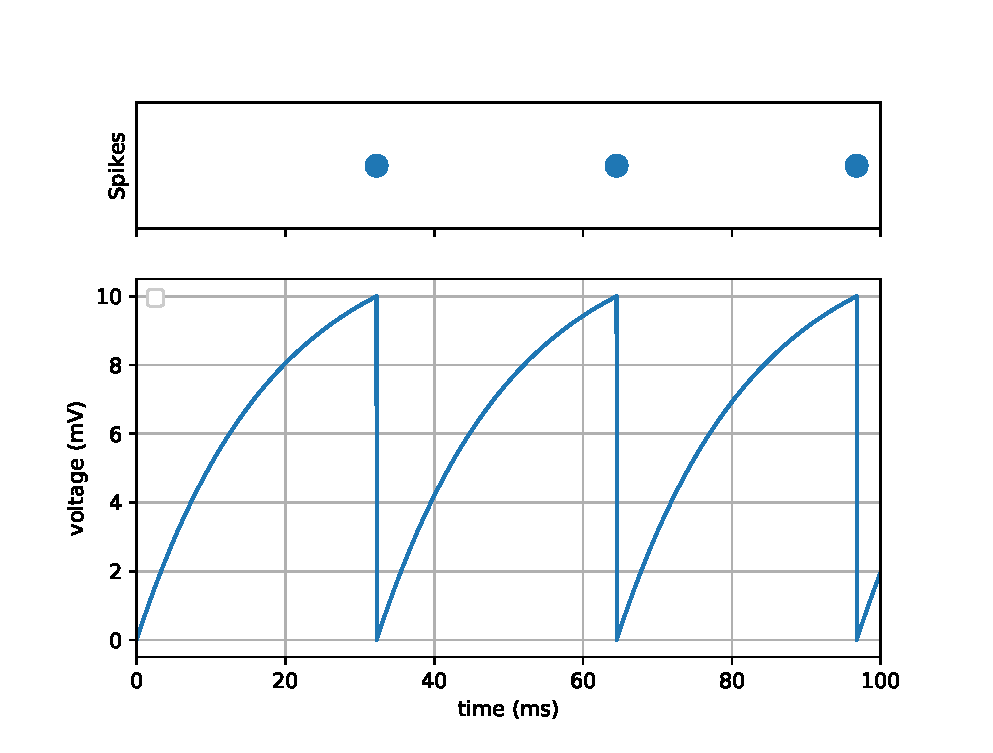
\includegraphics[width=1.0\linewidth]{figures/graphs/singleSpikingNeuron.eps}
        \caption{IF model}
        \label{fig:LIFSingleSpikeGraph}
    \end{subfigure}%
    \begin{subfigure}{.5\textwidth}
        \centering
        \includegraphics[width=1.0\linewidth]{figures/code/SingleLIFCode.png}
        \caption{IF Currents}
        \label{fig:LIFCode}
    \end{subfigure}
    \caption{Simulation of a single LIF neuron}
    \label{fig:LIFSingleSpikeGraphCode}
\end{figure}

The code is roughly based on example MATLAB code from \autocite[table
3.1]{trappenberg_fundamentals_2009} rewritten in idiomatic python. TODO explain
some rationale behind numbers and loop.

\begin{figure}[h!]
    \centering
    \addtolength{\leftskip} {-3cm}
    \addtolength{\rightskip}{-3cm}
    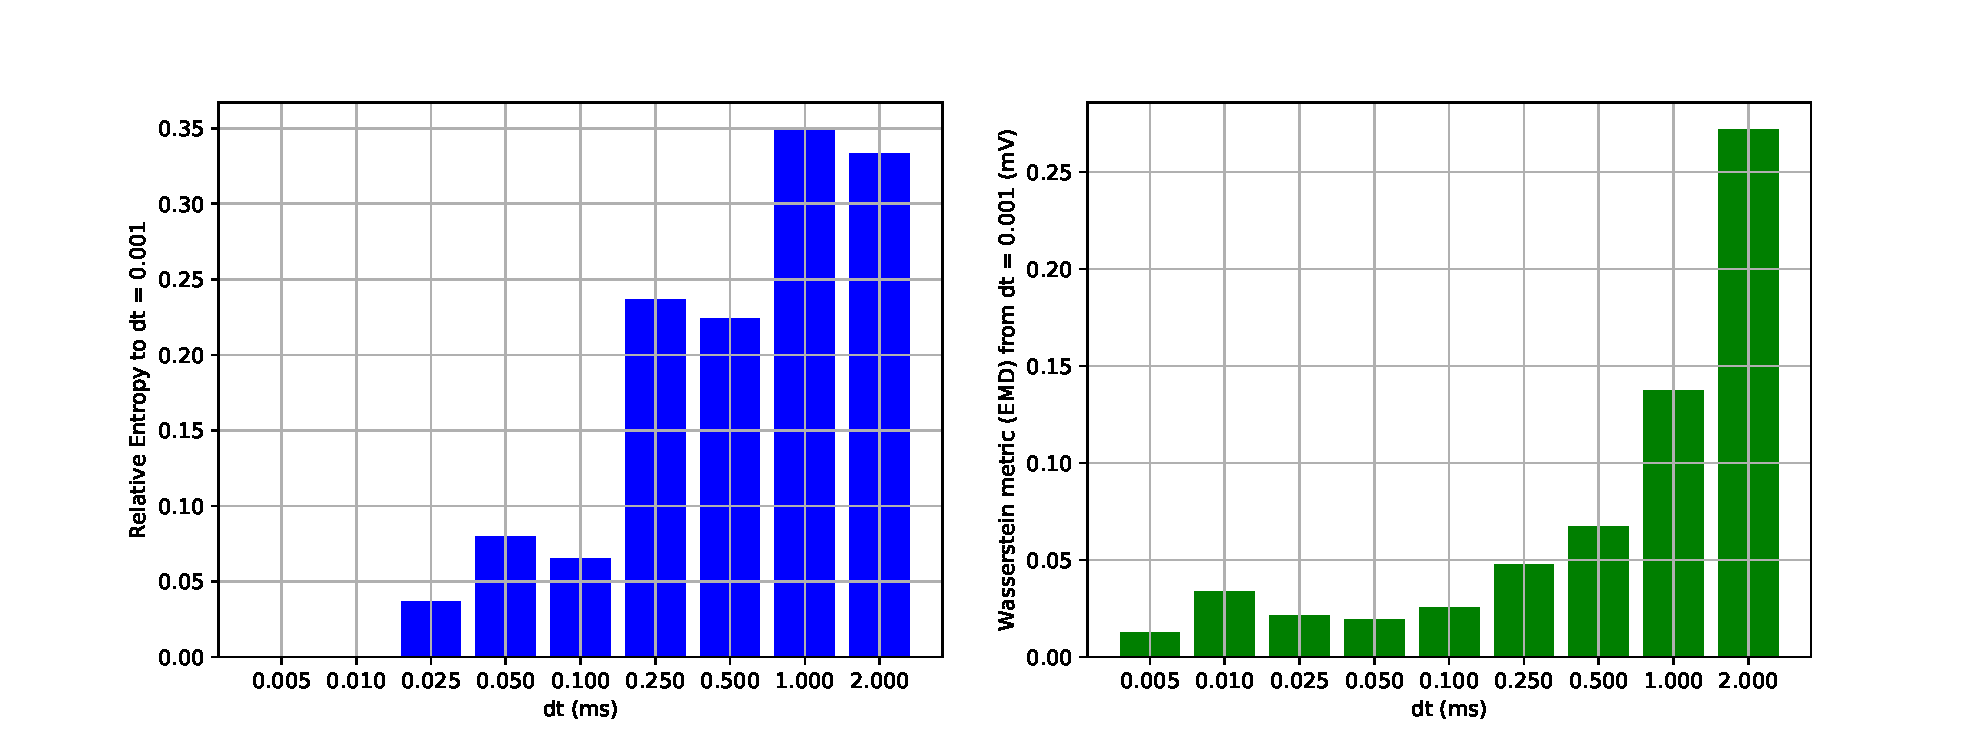
\includegraphics[width=1.4\linewidth]{figures/graphs/entropyofdt.eps}
    \caption{IF model with TODO}
    \caption{TODO}
    \label{fig:entropyofdt}
\end{figure}

Simulating a
neuron computationally requires integration, which means defining a suitably
small time-step $dt$ with which to perform descritization. The accuracy of
several $dt$ values is assessed in figure \ref{fig:entropyofdt}.

\begin{figure}[ht]
    \centering
    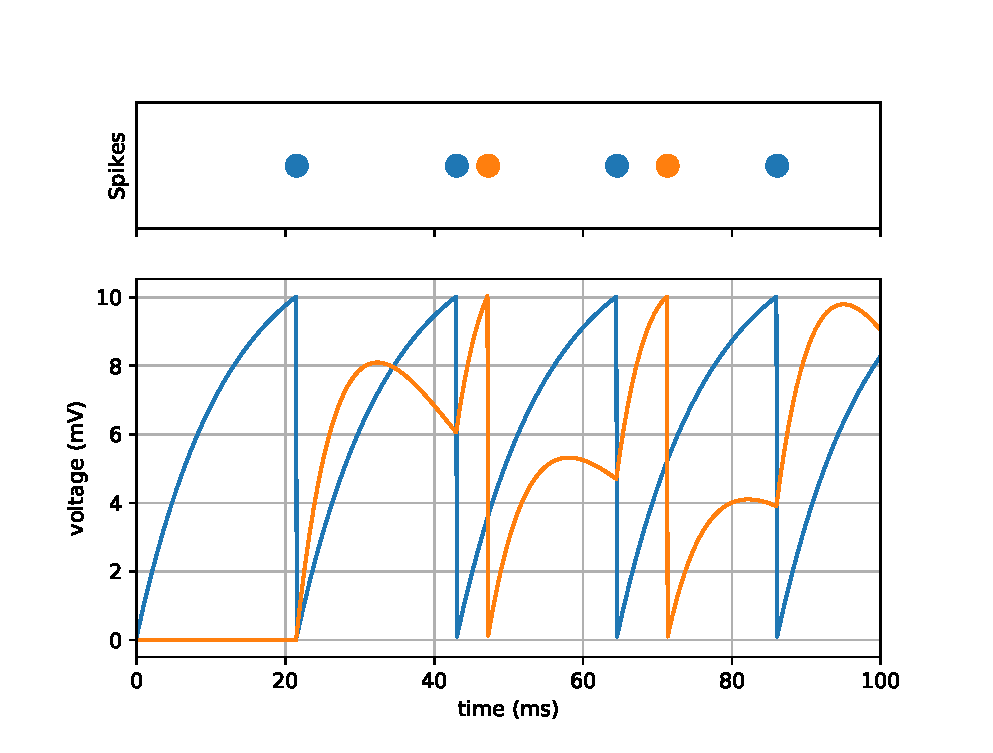
\includegraphics[width=.6\linewidth]{figures/graphs/dualSpikingNeuron.eps}
    \caption{IF model with TODO}
    \caption{TODO}
    \label{fig:LIFDoubleGraph}
\end{figure}



\pagebreak

% \subsection{Spike refractory periods}

% While the previously defined LIF neurons are sufficient for 

\subsection{Synapse mechanics}

Synapses between neurons effectively function as a gate, where the current that
passes through the gate decreases exponentially as time passes without any
pre-synaptic spikes. In general this relationship can be approximated by the
equation \ref{eq:Presynaptic1}, where the current across the synapse at a given
point is the product of the conductivity of the synapse channel $g_{syn}$ and the
reversal potential $E_{syn}$. As we are dealing solely with excitatory synapses in this
model, we can assume $E_{syn} = 0$.

\begin{equation}\label{eq:Presynaptic1}
    I_{syn} = g_{syn}(t)\cdot(v-E_{syn})
\end{equation}

The complexity of $g_{syn}$ that is required for a given model is different
depending on the intent. For this model it is necessary to implement basic
synaptic functionality, in particular, the delay between between the firing
time of a pre-synaptic neuron $t^f_{pre}$ and the point at which the channel
conductivity reacts to the spike. A simple formula for this is shown in figure
\ref{eq:Presynaptic2}, where only the most recent pre-synaptic firing time is
taken into account.

\begin{equation}\label{eq:Presynaptic2}
    g_{syn}(t) = \frac{q}{\tau_s}\cdot e^{-(\frac{t-t^f_{pre}}{\tau_s})}
\end{equation}

\subsection{STDP}

